\documentclass[runningheads]{llncs}
\usepackage[T1]{fontenc}
\usepackage{graphicx}
\usepackage{booktabs}
\newcommand{\corr}{\textsuperscript{*}}
% N.B.: do not change anything above this line. If you require additional
% packages, please load them directly after this line.
\usepackage[utf8]{inputenc}
\usepackage{amsmath}
\usepackage{amssymb}
\usepackage{multirow}
\usepackage[inline,shortlabels]{enumitem}
\usepackage[capitalize]{cleveref}
\newcommand{\citep}[1]{\cite{#1}}
\newcommand{\citet}[1]{\cite{#1}}

\newcommand{\thead}[1]{\begin{tabular}{@{}c@{}}#1\end{tabular}}

\begin{document}

\title{On the Role of Reversible Instance Normalization in Time Series Forecasting}
\titlerunning{On the Role of Reversible Instance Normalization in Time Series Forecasting}

\newif\ifanonymous
\anonymoustrue % submission
% \anonymousfalse % camera-ready

\ifanonymous
  \author{Anonymous Author(s)}
  \authorrunning{Anonymous Author(s)}
  \institute{Anonymous Institution}
\else
  % Current author, running-author, and institute blocks
  \author{Gaspard Berthelier\inst{1,2} \corr \and
    Tahar Nabil\inst{1} \and
    Etienne Le Naour\inst{1} \and
    Richard Niamke\inst{1} \and
    Samir Perlaza\inst{2} \and
    Giovanni Neglia\inst{2}}
    \authorrunning{G. Berthelier et al.}

    \institute{EDF R\&D, France\\
    \email{\{gaspard.berthelier,tahar.nabil,etienne.le-naour,richard.niamke\}@edf.fr}
    \and
    Inria Sophia Antipolis, France\\
    \email{\{samir.perlaza,giovanni.neglia\}@inria.fr}}
\fi


\maketitle

\begin{abstract}
Reversible Instance Normalization (RevIN) has become a common default in deep
time-series forecasting, although its gains are not universal. We ask a more
practical question: when is instance normalization preferable to global
standardization? We separate per-window normalization, RevIN's learnable affine
parameters, and normalized-space backpropagation in controlled ablations across
forecasting datasets, horizons, backbones, and random seeds. We evaluate both
future dates and unseen series and report seed uncertainty in addition to mean
error. The study shows how instance normalization trades robustness to offset
and scale heterogeneity against the loss of potentially predictive level and
scale information. This view explains why normalized-space training can help
on heterogeneous collections while global standardization remains competitive
on settings with limited shift, and motivates selecting normalization as an
experimental choice rather than treating RevIN as a universal default.

\keywords{Time series forecasting \and Instance normalization \and
Distribution shift}
\end{abstract}

\section{Introduction} \label{intro}

Data normalization is a fundamental preprocessing step, long recognized as essential for the stable and efficient training of neural networks. Its significance was established in early studies on neural networks optimization \citep{DBLP:series/lncs/LeCunBOM12}.
Normalization is particularly critical in time series forecasting, a domain in which deep learning models have achieved state-of-the-art performance \citep{patchtst}. Intrinsic properties of time series, such as non-stationarity, trends, and seasonality, introduce challenges that standard normalization methods fail to address \citep{adaptivenorm}.
%As a result, normalization becomes not merely a routine preprocessing step but a decisive factor influencing both model convergence and predictive performance.

Three major aspects must be considered when designing a normalization strategy for time series forecasting:

\begin{enumerate}[(i)]
    \item \textbf{Temporal distribution shift.} When training a neural forecaster over a training period, the input data distribution in a future test period may differ substantially. For instance, electricity consumption or road traffic often increase over time (see \cref{fig:shifts}).

    \item \textbf{Spatial distribution shift.} Neural forecasters are typically trained on multiple time series and must generalize to unseen time series at inference. Even when series describe similar phenomena (e.g., solar power generation at different locations), their overall distributions may differ, for example, due to scale or level shifts (see \cref{fig:shifts}).

    % \item \textbf{Conditional distribution shift.} A neural forecaster maps a look-back window to a horizon window, $f_{\theta}: \boldsymbol{x}^{\text{look-back}} \to \boldsymbol{x}^{\text{horizon}}$. The conditional distribution $p(\boldsymbol{x}^{\text{horizon}} | \boldsymbol{x}^{\text{look-back}})$ may vary both in space and time. This shift remains particularly challenging to handle (see \cref{fig:c}).
    \item \textbf{Conditional distribution shift.} A neural forecaster maps past \textit{look-back} windows to future \textit{horizon} windows. The conditional distribution of the horizon given the look-back may vary both in space and time. This shift remains particularly challenging to handle (see \cref{fig:shifts}).
\end{enumerate}



\begin{figure}[t]
    \centering
    \begin{minipage}[t]{0.31\textwidth}
        \centering
        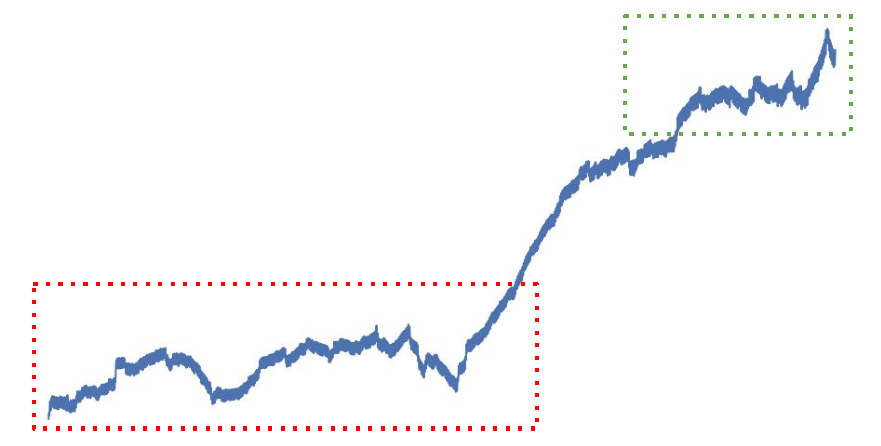
\includegraphics[width=\linewidth]{Images/misc/temporal_shift_traffic.pdf}\\
        (a) Temporal shift.
    \end{minipage}
    \hfill
    \begin{minipage}[t]{0.31\textwidth}
        \centering
        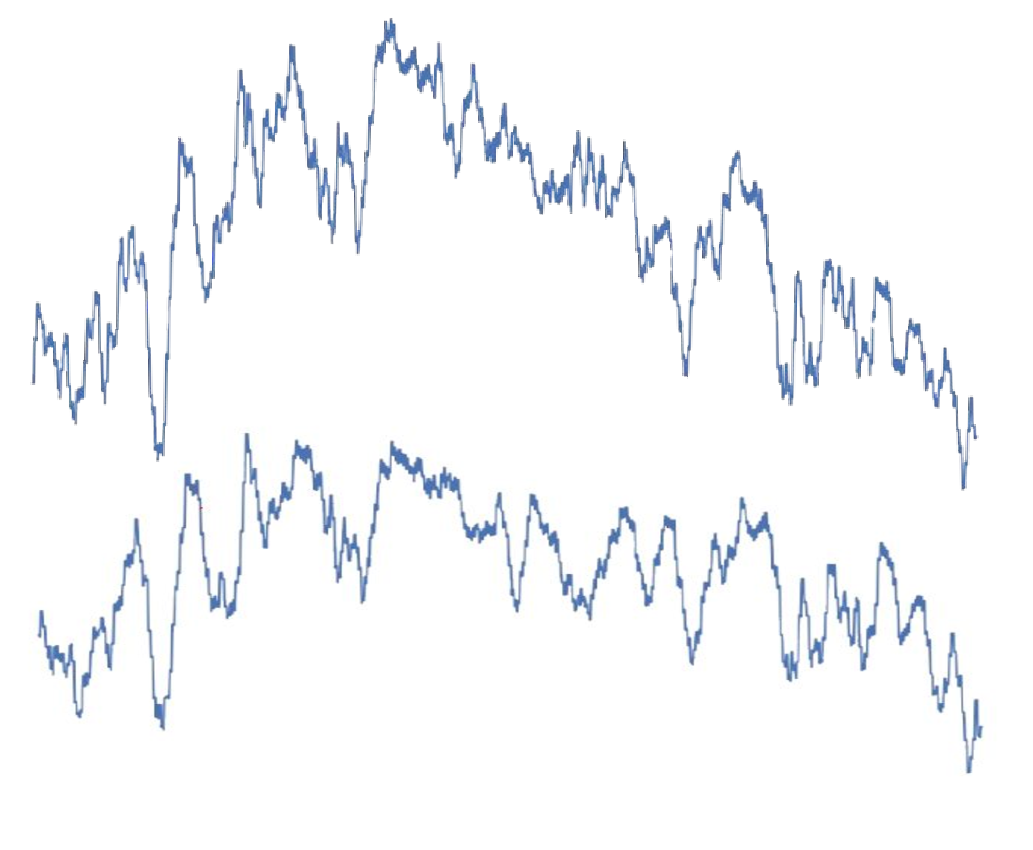
\includegraphics[width=\linewidth]{Images/misc/solar_distrib_shift.pdf}\\
        (b) Spatial shift.
    \end{minipage}
    \hfill
    \begin{minipage}[t]{0.31\textwidth}
        \centering
        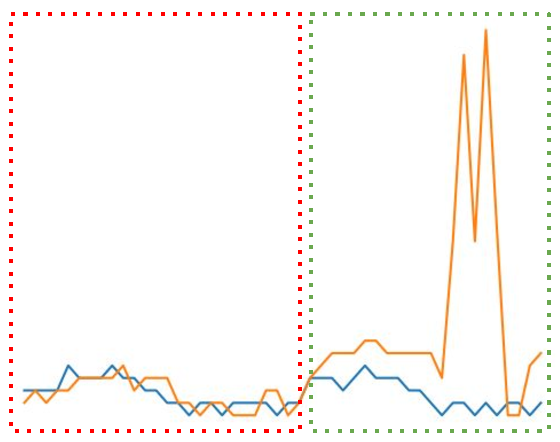
\includegraphics[width=\linewidth]{Images/misc/cond_shift_ecl.pdf}\\
        (c) Conditional shift.
    \end{minipage}
    \caption{Illustration of the three distribution shifts: (a) temporal
    shift between training and test periods (rolling average of a
    \textsc{Traffic} sensor), (b) spatial shift between users (two
    \textsc{Solar} sensors), and (c) conditional shift (different horizons
    for similar look-back windows from one \textsc{Electricity} user).}
    \label{fig:shifts}
\end{figure}


%\clearpage

In deep learning, a common approach is to apply \textit{standard normalization} to all data points, using a single global mean $\mu$ and standard deviation $\sigma$ computed empirically over the training data. Each data point is processed by subtracting the mean and dividing by the standard deviation. However, this global normalization fails to address the challenges of the three distribution shifts
%(i), (ii) and (iii)
described above
\citep{adaptivenorm}. Indeed, the statistics estimated on the training data may no longer be valid at inference. A more sophisticated and widely adopted normalization strategy is \textit{instance normalization}, which normalizes input windows using their individual statistics. This ensures that whatever the scale and offset of the input, all windows seen by the model will be similarly distributed. This method was introduced to the forecasting community as \textit{Reversible Instance Normalization} (RevIN) \citep{revin}.

The RevIN method has been adopted in numerous recent forecasting studies \citep{patchtst,fits,tirex,HUANG2025114036,revin}. Its authors argue that RevIN mitigates the distribution shift problem in time series. In this work, we investigate this claim more closely.
Our contributions are summarized as follows:
\begin{itemize}
    \item We review normalization techniques for neural forecasters and identify the key challenges they face in time series applications.
    \item We conduct extensive ablation studies on RevIN using standard forecasting benchmarks and show which components are truly necessary.
    \item We discuss the effects of instance normalization on input and output data distributions and highlight the limitations of RevIN.
    % \item We claim the \textit{conditional shift between look-back and horizon windows} remains an open challenge, and draw perspectives on how to address it.
\end{itemize}

\newpage
\section{Setting}

In this section, we formally introduce the task of time series forecasting and the distributional challenges it faces.

\paragraph{Time Series Forecasting} The task of time series forecasting consists in finding an optimal parameterized model $f_\theta$ of the form:
\begin{equation}
\label{eq:definition}
f_\theta:\;
\begin{array}{@{}c@{~}c@{~}l@{}}
  \mathbb{R}^{L} & \longrightarrow & \mathbb{R}^{H}, \\
x & \longmapsto & \hat{y} \approx y,
\end{array}
\qquad
\begin{aligned}
L &:\ \text{look-back window size},\\
H &:\ \text{horizon size}.
\end{aligned}
\end{equation}
where $\theta$ denotes the parameters of the model (e.g. a neural network), fitted on a training dataset $\mathcal{D}$ of $N$ pairs of windows $(x, y)$, with $x$ a past look-back window and $y$ a horizon to forecast. Naturally, the goal is to have predictions $\hat{y}=f_{\theta}(x)$ as close as possible to the ground-truth horizons $y$. We say a model \textit{generalizes} well when this is the case for unseen windows.

Equation \ref{eq:definition} corresponds to the \textit{univariate regression} setting, considered in this paper. A more general formulation could include multivariate inputs and outputs, exogenous covariates, and probabilistic predictions; nevertheless, we expect the main conclusions to carry over to these settings.
%, we do not consider it here.

\paragraph{Distribution shifts}
Formally, let $\mathcal{P}^{\mathcal{I},\mathcal{T}}_{X,Y}$ denote the distribution of windows corresponding to series (users / sensors) $\mathcal{I}$, during the time period $\mathcal{T}$. Temporal and spatial shifts occur when the marginal distribution $\mathcal{P}^{\mathcal{I},\mathcal{T}}_{X}$ varies across different time periods in $\mathcal{T}$ and different users in $\mathcal{I}$, respectively. They are particular examples of \textit{covariate shift} \citep{kairouz2021advances} as they describe changes in input distributions. Conditional shift occurs when the conditional distribution
$\mathcal{P}^{\mathcal{I},\mathcal{T}}_{Y|X}$ varies across $\mathcal{I}$ or $\mathcal{T}$.  It corresponds to a \textit{concept drift} \citep{moreno2012unifying}, and describes a change in the expected output for a given input. When learning a forecasting model, we typically sample examples from a subset of users $\mathcal{I}_{train}$ and a fixed time period $\mathcal{T}_{train}$. We refer to generalization as the capacity of the model to perform well for new users $\mathcal{I}_{test}$ and at a future time period $\mathcal{T}_{test}$. In case of temporal, spatial, and conditional shifts, input normalization aims to improve generalization.

\section{Normalization for Time Series Forecasting} \label{related-content}

\paragraph{Global normalization.}
Standard normalization uses statistics estimated over the training data:
\begin{equation}
    \tilde{x}=\frac{x-\mu}{\sigma+\epsilon}, \qquad
    \mu=\frac{1}{N}\sum_{x\in\mathcal{D}}\frac{1}{L}\sum_{i=1}^Lx_i.
\end{equation}
It improves numerical conditioning, but the fixed statistics may cease to
describe future dates or unseen series. Related normalization layers vary the
dimensions and population used to estimate statistics; BatchNorm
\citep{batchnorm}, LayerNorm \citep{layernorm}, and GroupNorm
\citep{groupnorm} are familiar examples. In this work, we focus on input
normalization rather than hidden-layer normalization.

\paragraph{Reversible instance normalization.}
Drawing on instance normalization \citep{instancenorm}, RevIN \citep{revin}
computes statistics independently for each look-back window:
\begin{equation}
\mu_x = \frac{1}{L}\sum_{i=1}^L x_i, \qquad
\sigma_x^2 = \frac{1}{L}\sum_{i=1}^L(x_i-\mu_x)^2.
\end{equation}
For a forecaster $f_\theta$, its affine version applies
\begin{equation}
\tilde{x}=\alpha\frac{x-\mu_x}{\sigma_x+\epsilon}+\beta,
\qquad
\hat{y}=(\sigma_x+\epsilon)
\frac{f_\theta(\tilde{x})-\beta}{\alpha+\epsilon}+\mu_x.
\end{equation}
The pipeline standardizes a look-back, applies global learnable parameters
$(\alpha,\beta)$, forecasts, reverses the affine transform, and returns to data
space. \Cref{fig:revin-process} illustrates these steps.

\begin{figure}[h!]
    \centering
    \vspace{-5mm}
    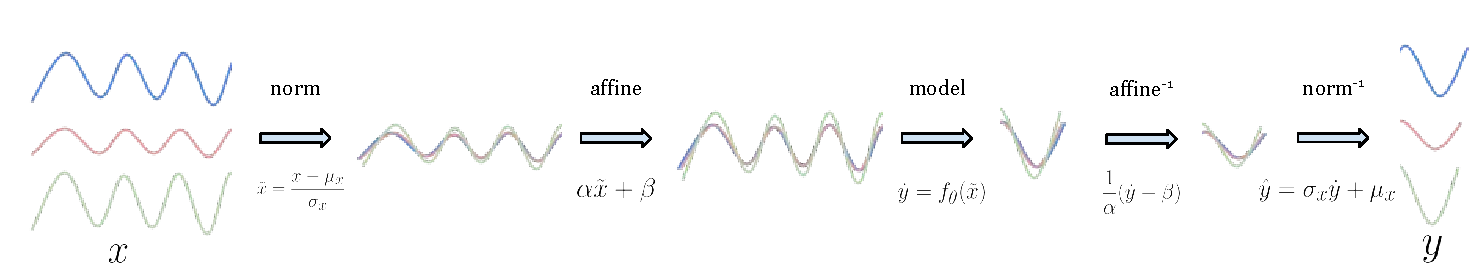
\includegraphics[width=\linewidth]{Images/min/illustrated_revin.pdf}
    \vspace{-5mm}
    \caption{Illustration of the RevIN process on three synthetic examples.}
    \label{fig:revin-process}
\end{figure}

\paragraph{The central trade-off.}
Per-window normalization guarantees zero input mean and unit input variance
before the optional affine layer. This can remove nuisance offset and scale
differences across dates and series. However, two windows that differ only in
absolute level or scale then become indistinguishable to the backbone. Instance
normalization should therefore help when those statistics vary across domains
without changing the normalized forecasting relationship, and can hurt when
they carry predictive information. Our experiments isolate this trade-off and
the separate optimization effect of weighting errors in normalized space; we
do not introduce a new normalization architecture.

\section{When Is Instance Normalization Useful?} \label{ablation-studies}

\subsection{Controlled benchmark} \label{quantitative}

\paragraph{Compared components.}
We compare no normalization, global standardization, non-affine instance
normalization, and affine RevIN. For the two instance-normalized variants, we
also compare data-space MSE with normalized MSE,
\begin{equation}
 \mathcal{L}_{\mathrm{nMSE}}(\hat y,y\mid x)
 =\frac{1}{H}\sum_{h=1}^{H}
 \left(\frac{\hat y_h-y_h}{\sigma_x+\epsilon}\right)^2.
\end{equation}
Predictions are always returned to data space and evaluated with ordinary MSE;
normalized MSE only changes the weight assigned to each training window. This
factorial comparison separates the forward normalization, RevIN's affine
parameters, and scale-balanced optimization.

\paragraph{Datasets and splits.}
The expanded benchmark uses \textsc{ETTh1}, \textsc{Electricity},
\textsc{Traffic}, \textsc{Solar}, \textsc{Weather}, and
\textsc{Exchange Rate}. Dates are split sequentially into train, validation,
and test periods. Series are independently split into seen and unseen groups.
Models are trained on seen series in the training period and evaluated on
future dates for seen series (Test1) and future dates for unseen series (Test2).
We study $(L,H)$ in
\[
\{(168,24),(168,168),(504,24),(504,168),(504,504),
  (720,168),(720,720)\}.
\]

\paragraph{Protocol.}
We use \textsc{PatchTST} \citep{patchtst} and \textsc{DLinear}
\citep{dlinear}. Training samples random users and window starts, uses Adam
\citep{adam}, batch size 256, learning rate $10^{-5}$, and five seeds.
Every run uses exactly 10,000 optimizer steps. Validation is evaluated every
1,000 optimizer steps; evaluation windows use a
horizon-sized stride. Every table reports seed mean $\pm$ sample standard
deviation, while run summaries retain the variance and count of per-point loss
contributions. The rewritten implementation is first checked in short test mode
and then compared with the earlier results before the expanded analysis is
used.

% The bundled table is the previous three-dataset reproduction target. Once the
% new full run is complete, replace it with the generated mean-plus-uncertainty
% tables under outputs/revin_experiment/.
\begin{table}[t]
\caption{Ablation of RevIN components on \textsc{PatchTST} (MSE on new dates). Average improvements are reported relative to the no-normalization baseline. BP stands for ``backpropagation", Std. for "standard". In bold: best models per settings (rows).}
\centering
\setlength{\tabcolsep}{1.5pt}
\begin{tabular}{lccccccc}
\toprule
& & & & \multicolumn{2}{c}{RevIN (w/o $\alpha,\beta$)} & \multicolumn{2}{c}{RevIN} \\
     \cmidrule(r){5-6} \cmidrule(r){7-8}
 & L-H & None & Std. norm. & \thead{Std.\\BP} & \thead{Norm.\\BP} & \thead{Std.\\BP} & \thead{Norm.\\BP} \\
\midrule
\multirow{4}{*}{Electricity} & 168-24 & 349.83 & 20.56 & 8.52 & \textbf{4.91} & 8.52 & 4.92 \\
 & 504-24 & 348.14 & 19.68 & 8.36 & \textbf{4.09} & 8.34 & 4.09 \\
 & 504-168 & 347.21 & 28.28 & 11.00 & \textbf{7.09} & 10.94 & \textbf{7.09} \\
 & 504-504 & 358.70 & 33.18 & 16.70 & 12.54 & 16.65 & \textbf{12.53} \\
\midrule
\multirow{4}{*}{Solar} & 168-24 & 3.05 & 2.30 & 1.47 & \textbf{1.46} & 1.47 & 1.47 \\
 & 504-24 & 3.12 & 2.16 & 1.44 & \textbf{1.38} & 1.44 & 1.38 \\
 & 504-168 & 2.81 & 3.19 & 2.22 & \textbf{2.18} & 2.22 & \textbf{2.18} \\
 & 504-504 & 2.82 & 3.55 & 2.40 & \textbf{2.33} & 2.40 & \textbf{2.33} \\
\midrule
\multirow{4}{*}{Traffic} & 168-24 & 15.74 & \textbf{6.96} & 8.10 & 8.07 & 8.10 & 8.07 \\
 & 504-24 & 19.62 & \textbf{6.44} & 7.52 & 7.47 & 7.52 & 7.47 \\
 & 504-168 & 19.85 & \textbf{7.10} & 8.39 & 8.36 & 8.38 & 8.35 \\
 & 504-504 & 19.10 & \textbf{7.17} & 8.49 & 8.47 & 8.48 & 8.47 \\
\midrule
\multirow{3}{*}{Synthetic} & 40-10 & $3.4\times10^{6}$ & $1.5\times10^3$ & 4.28 & \textbf{4.27} & 4.28 & \textbf{4.27} \\
 & 100-20 & $3.2\times10^{6}$ & $5.3\times10^{3}$ & 3.66 & 3.66 & \textbf{3.65} & \textbf{3.65} \\
 & 100-100 & $3.2\times10^{6}$ & $9.8\times10^{3}$ & \textbf{4.25} & \textbf{4.25} & \textbf{4.25} & \textbf{4.25} \\
\midrule
Improvements &  & 0.0 $\%$ & 62.32 $\%$ & 70.1 $\%$ & \textbf{70.84} $\%$ & 70.11 $\%$ & 70.84 $\%$ \\
\bottomrule
\end{tabular}
\label{tab:main1}
\end{table}

\begin{table}[t]
\caption{Ablation of RevIN components on \textsc{PatchTST} (MSE on new dates and new users). Average improvements are expressed relative to the first column. BP stands for ``backpropagation", Std. for "standard". In bold: best models per settings (rows).}
\centering
\setlength{\tabcolsep}{1.5pt}
\begin{tabular}{lccccccc}
\toprule
& & & & \multicolumn{2}{c}{RevIN (w/o $\alpha,\beta$)} & \multicolumn{2}{c}{RevIN} \\
     \cmidrule(r){5-6} \cmidrule(r){7-8}
 & L-H & None & Std. norm. & \thead{Std.\\BP} & \thead{Norm.\\BP} & \thead{Std.\\BP} & \thead{Norm.\\BP} \\
\midrule
\multirow{4}{*}{Electricity} & 168-24 & 61.16 & 23.55 & 0.93 & \textbf{0.59} & 0.93 & \textbf{0.59} \\
 & 504-24 & 60.82 & 22.32 & 0.92 & \textbf{0.52} & 0.92 &\textbf{ 0.52} \\
 & 504-168 & 60.27 & 21.33 & 1.02 & \textbf{0.67} & 1.01 & \textbf{0.67} \\
 & 504-504 & 60.82 & 23.04 & 1.23 & \textbf{0.87} & 1.22 & \textbf{0.87} \\
\midrule
\multirow{4}{*}{Solar} & 168-24 & 2.74 & 2.35 & 1.31 & \textbf{1.30} & 1.31 & \textbf{1.30} \\
 & 504-24 & 2.74 & 2.20 & 1.28 & \textbf{1.23} & 1.28 &\textbf{ 1.23} \\
 & 504-168 & 2.54 & 3.24 & 1.97 & \textbf{1.94} & 1.97 & \textbf{1.94} \\
 & 504-504 & 2.52 & 3.59 & 2.13 & \textbf{2.06} & 2.13 & 2.07 \\
\midrule
\multirow{4}{*}{Traffic} & 168-24 & 14.44 & \textbf{6.51} & 7.30 & 7.27 & 7.30 & 7.27 \\
 & 504-24 & 19.60 & \textbf{6.02} & 6.77 & 6.72 & 6.77 & 6.72 \\
 & 504-168 & 18.75 & \textbf{6.87} & 8.13 & 8.09 & 8.13 & 8.09 \\
 & 504-504 & 17.87 & \textbf{6.99} & 8.29 & 8.26 & 8.28 & 8.25 \\
\midrule
\multirow{3}{*}{Synthetic} & 40-10 & $3.6\times10^{6}$ & $1.5\times10^{3}$ & \textbf{4.30} & \textbf{4.30} & \textbf{4.30} & \textbf{4.30} \\
 & 100-20 & $3.3\times10^{6}$ & $5.6\times10^{3}$ & \textbf{3.68} &\textbf{ 3.68} & \textbf{3.68} & \textbf{3.68} \\
 & 100-100 & $3.3\times10^{6}$ & $1.1\times10^{4}$ & \textbf{4.30} & \textbf{4.30} & \textbf{4.30} & \textbf{4.30} \\
\midrule
Improvements &  & 0.0 $\%$  & 6.97 $\%$   & 70.62 $\%$   & \textbf{71.29} $\%$   & 70.63 $\%$   & \textbf{71.29} $\%$   \\
\bottomrule
\end{tabular}
\label{tab:main2}
\end{table}


\paragraph{Reproduction hypotheses.}
The previous implementation suggested three findings to verify rather than
assume. First, normalized-space training improved data-space MSE on the more
heterogeneous collections. Second, the learnable affine parameters added little
over non-affine instance normalization. Third, global standardization remained
better on \textsc{Traffic}. The expanded dataset, horizon, backbone, and seed
sweep tests whether these observations are stable or dataset-specific.

\subsection{Relating gains to heterogeneity} \label{qualitative}

Instance normalization directly removes variation in look-back location and
scale. If $\mathcal{P}_{\mathrm{train}}$ and
$\mathcal{P}_{\mathrm{test}}$ denote input-window distributions, its most
plausible benefit is therefore in settings with shifts such as
\begin{equation}
 \mathbb{E}_{x\sim\mathcal{P}_{\mathrm{train}}}[\mu_x]
 \neq \mathbb{E}_{x\sim\mathcal{P}_{\mathrm{test}}}[\mu_x],
 \qquad
 \mathbb{E}_{x\sim\mathcal{P}_{\mathrm{train}}}[\sigma_x]
 \neq \mathbb{E}_{x\sim\mathcal{P}_{\mathrm{test}}}[\sigma_x].
\end{equation}
This is only a limited form of distribution alignment: higher-order structure,
frequency content, and dynamics may still differ. Conversely, removing
$(\mu_x,\sigma_x)$ is harmful when absolute level or scale helps predict the
horizon.

As a descriptive diagnostic, we compute energy distance
\citep{smola2006maximum} between train and test inputs,
\begin{equation}
d^2_{\mathrm{energy}}(P,Q)=
\mathbb{E}_{P,P}[k(x,x')]+\mathbb{E}_{Q,Q}[k(y,y')]
-2\mathbb{E}_{P,Q}[k(x,y)],
\quad k(x,y)=-\lVert x-y\rVert_2.
\end{equation}
These distances and the t-SNE visualizations \citep{tsne} are computed in a
separate dataset-analysis notebook, independently of model training. They are
used to test association with forecasting gains, not as evidence of causality.

\begin{table}[t]
\caption{Previously computed energy distances between input distributions.
T and S vary time periods and series, respectively. Values will be recomputed
with the expanded benchmark splits.}\label{tab:distances}
\centering
\setlength{\tabcolsep}{3pt}
\begin{tabular}{lrrrrrr}
\toprule
& \multicolumn{2}{c}{None} & \multicolumn{2}{c}{Standard}
& \multicolumn{2}{c}{Instance}\\
\cmidrule(lr){2-3}\cmidrule(lr){4-5}\cmidrule(lr){6-7}
& T & S & T & S & T & S\\
\midrule
Electricity & 7.09 & 57.16 & \textbf{0.05} & \textbf{0.42} & 0.64 & 1.01\\
Solar       & 3.48 & 0.98  & 1.05 & 0.30 & \textbf{0.78} & \textbf{0.29}\\
Traffic     & \textbf{0.32} & 0.99 & 1.39 & 4.29 & 0.92 & \textbf{0.45}\\
\bottomrule
\end{tabular}
\end{table}

\begin{figure}[t]
\centering
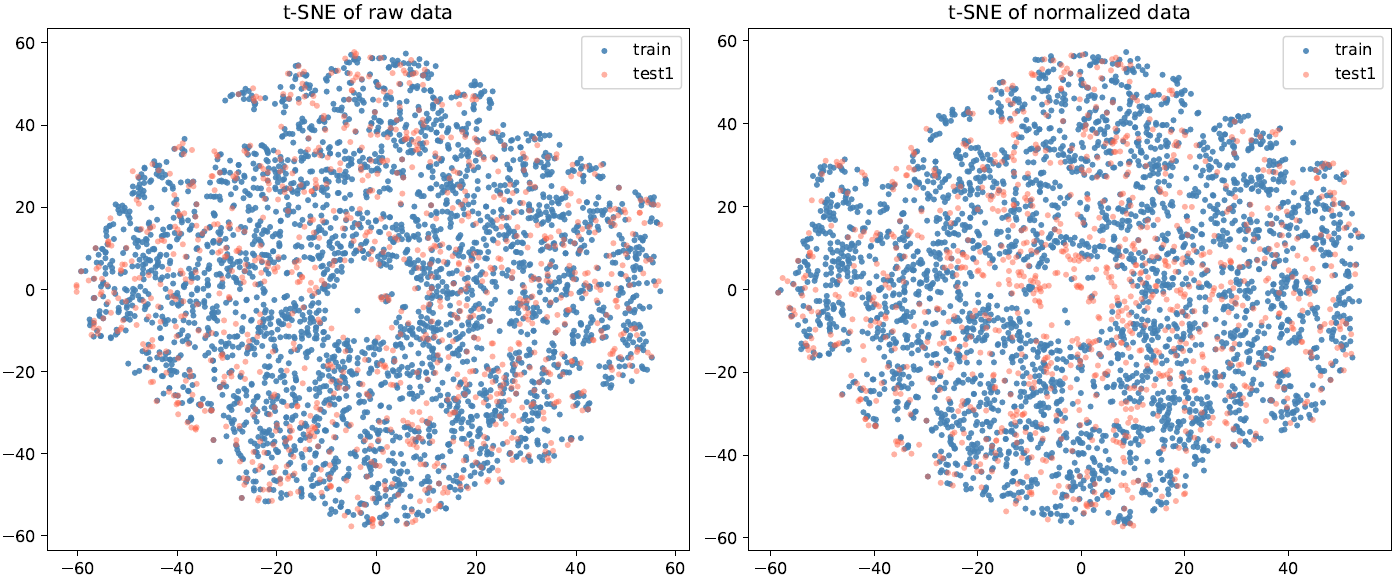
\includegraphics[width=0.7\linewidth]{Images/tsne/traffic_time_tsne.png}
\caption{Previous t-SNE embeddings of \textsc{Traffic} train (blue) and test
(orange) inputs before (left) and after (right) instance normalization.}
\label{fig:traffic_time_tsne}
\end{figure}

\subsection{Normalization choice as an oracle reference}

Raw MSEs are not directly comparable across datasets with different units. We
therefore report both the equal-configuration macro average
\begin{equation}
 \overline{M}(m)=\frac{1}{|\mathcal{C}|}
 \sum_{c\in\mathcal{C}}M_{c,m}
\end{equation}
and the mean per-setting relative gain over global standardization. In addition
to fixed standard, non-affine instance, and affine RevIN policies, we compute a
test oracle that chooses between standard normalization and full affine RevIN
for each dataset--setting pair. This oracle is an
optimistic upper reference, not a valid deployment procedure, because it uses
test outcomes for selection. Its gap to either fixed policy nevertheless
quantifies how much could be gained by learning a normalization-selection rule
from pre-test diagnostics. All policy comparisons use the same complete seeds
and report the standard deviation and variance of seed-level macro averages.

\section{Conclusion} \label{conclu}

Instance normalization is best understood as a conditional experimental choice,
not a universal forecasting default. It removes look-back offset and scale,
which can improve robustness when those quantities vary across dates or series
without changing the normalized forecasting relationship. The same operation
can be detrimental when absolute level and scale are predictive. Normalized
backpropagation adds a separate effect by balancing gradient contributions from
series with different scales, while RevIN's symmetric affine parameters must be
judged independently.

Our expanded protocol tests these mechanisms across datasets, horizons,
backbones, future dates, unseen series, and random seeds. Reporting seed
uncertainty and within-run error variance is essential because small average
gains may otherwise be indistinguishable from training variability. Finally,
the standard-versus-RevIN oracle measures the headroom available from
choosing normalization per setting, while remaining explicitly optimistic.
Together, these analyses aim to replace the blanket question ``does RevIN
work?'' with the more useful question ``under which data conditions does
instance normalization help?''


\begin{credits}
\subsubsection{\discintname}
The authors have no competing interests to declare that are relevant to
the content of this article.
\end{credits}

\bibliographystyle{splncs04}
\bibliography{biblio}

\end{document}
